\chapter{Projekt systemu}
\thispagestyle{chapterBeginStyle}

{\color{dgray}
W tym rozdziale przedstawiono szczegółowy projekt systemy w notacji UML uwzględniający wymagania funkcjonalne opisane w rozdziale~\ref{rozdzial1}. Do opisu relacji pomiędzy składowymi systemu wykorzystano diagramy \ldots.
Przedstawiono w pseudokodzie i omówiono algorytmy generowania \ldots.
}


\section{Grupy użytkowników i założenia}


\section{Przypadki użycia}
Jak zostało zdefiniowane w poprzednim punkcie, w pracy przewidziano 3 grupy użytkowników. W zamyśle framework jest narzędziem dla programisty, jednak w systemie został zaimplementowany szereg rozwiązań gotowych do wykorzystania dla końcowych użytkowników, dlatego diagramy przypadków użycia zostały podzielone na trzy klasy: 
\begin{itemize}
	\item przypadki użycia Programisty 
	\item przypadki użycia Użytkownika Administracyjnego potencjalnego serwisu e-commerce, opartego na opisywanym Frameworku
	\item przypadki użycia użytkownika końcowego, czyli Klienta
\end{itemize}
Na rysunku \ref{useCaseProgrammer} zostały przedstawione najważniejsze przypadki użycia frameworku. Programista ma swobodny dostęp do rozszerzania encji, w szczególności klasy Produkt, która ma wyjatkowo strategiczne znaczenie w systemach e-commerce. Dodatkowo ma możliwość uczynienia niestandardowych pól wyszukiwalnymi przez klienta. Sytuacja została zobrazowana na poniższym przykładzie.
\begin{example}
	Załóżmy, że mamy niestandardowe pole proste (String) w encji klasyfikowanej przez twórców ewentualnego sklepu związanego z opisywanym frameworkiem jako finalna encja nadająca się do sprzedaży. Niech nazywa się \texttt{MyProduct extends Product} z polem \texttt{myCustomField}. Jedyne co w tej sytuacji musimy zrobić aby system mógł wyciągnąć wartość tego pola z encji (o której de facto nie wie) to wpisać do tabeli zawierającej indeksowane cechy produktu nazwę danego pola, system za pomocą refleksji\footnote{\textit{refleksja} ( eng. reflection) -- udogodnienie w języku Java, pozwalające na wyświetlenie i manipulacje właściwościami klasy. Więcej w sekcji \textbf{słowniczek}.} wyekstaktuje wartość pola z encji.    
\end{example}
\begin{figure}
	\begin{center}
		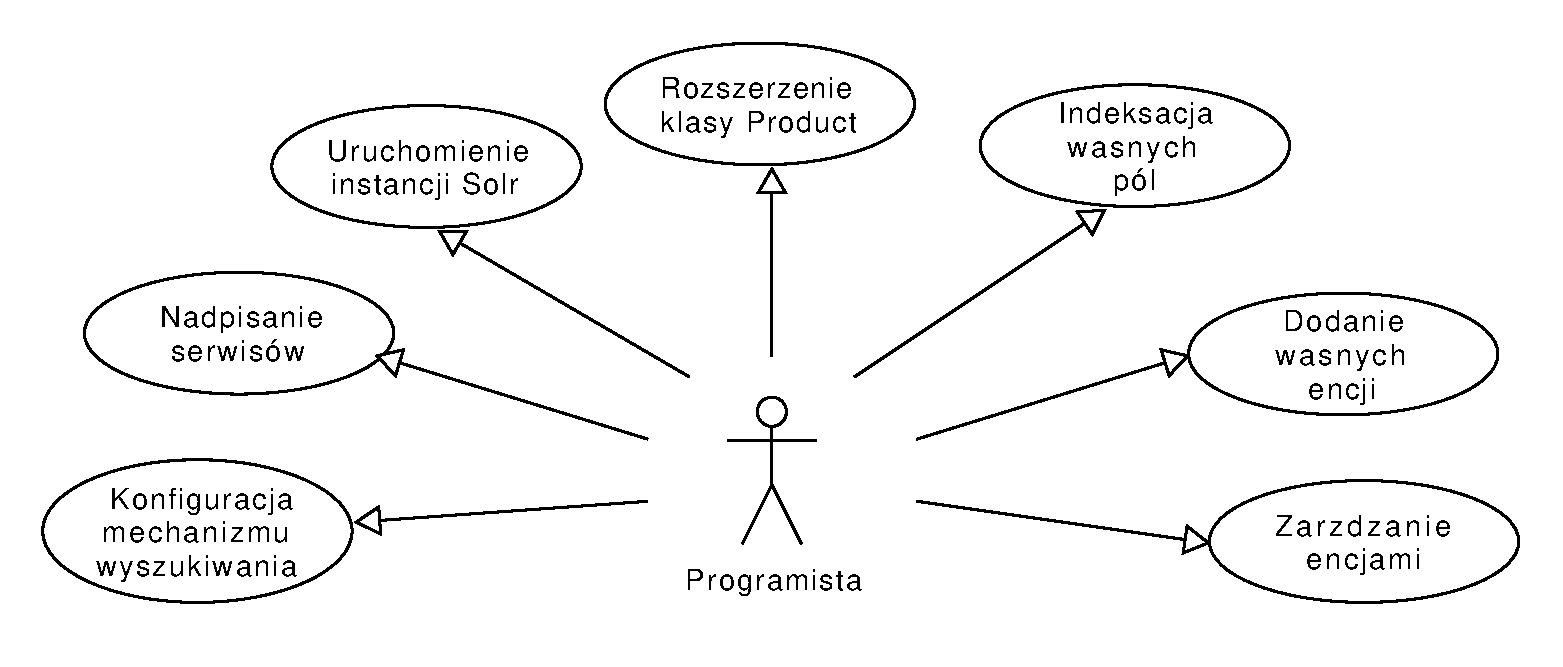
\includegraphics[width=1\textwidth]{ucdev.pdf}
	\end{center}
	\caption{{\color{black}Diagram przypadków użycia związany z Programistą.}} \label{useCaseProgrammer}
\end{figure}
\begin{figure}
	\begin{center}
		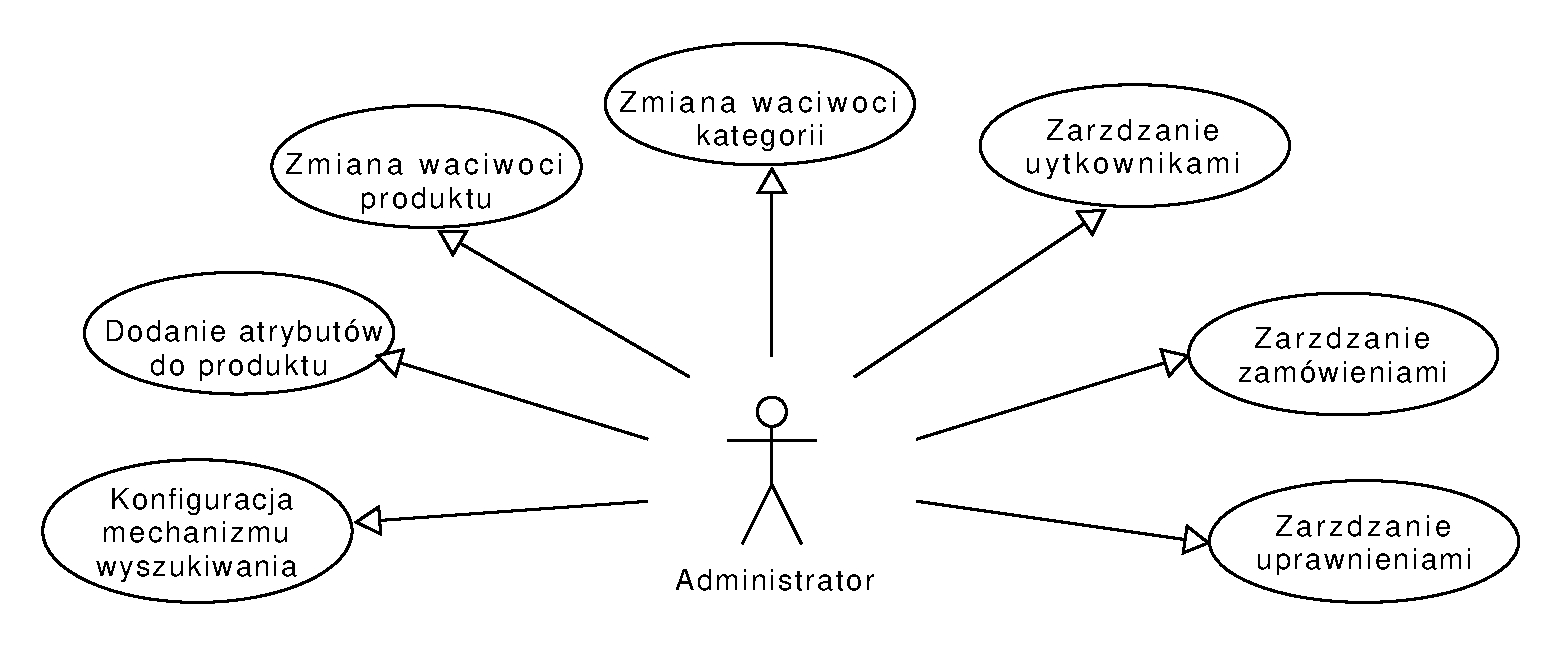
\includegraphics[width=1\textwidth]{ucadmin.pdf}
	\end{center}
	\caption{{\color{black}Diagram przypadków użycia związany z Administratorem ewentualniego systemu.}} \label{useCaseAdmin}
\end{figure}
Dodane przez Programistę encje są obsługiwane przez framework, dodatkowo po dodaniu specjalnej adnotacji\footnote{adnotacja -- używane w języku Java od wersji 1.7, najczęściej służą do określania dodatkowych właściwości pól bądź klas} nad nią, może być zarządzana w uniwersalnym panelu administracyjnym. Osoba zajmująca się implementacją sklepu opartego o opisywaną platformę może uruchomić dowolną \textit{(skończoną)} ilość instancji Apache Solr, czyli bazy danych noSQL, służącej do obsługiwania zapytań związanych z katalogiem produktowym (skalowalność pionowa tylko tej części aplikacji, która tego potrzebuje). W odniesieniu do przypadku użycia \textit{Nadpisanie mechanizmu wyszukiwania} z rysunku \ref{useCaseProgrammer} serwisy są oparte na interfejsach, zapewniając Programiście możliwość nadpisania jego logiki zgodnie z zasadami polimorfizmu. 

Rysunek \ref{useCaseAdmin} przedstawia przypadki użycia z punktu widzenia Administratora potencjalnego systemu. Z punktu widzenia platformy jest to również klient, gdyż framework zakłada, że nie ma on wiedzy technicznej i nie potrafi programować. Podobnie jak programista, może konfigurować mechanizm wyszukiwania, jednak bardziej wysokopoziomowo, np. deklaracja używanych facetów. Panel administracyjny zakłada zarządanie najważniejszymi encjami: produkt, kategoria, użytkownik, zamówienie, uprawnienie i parę innych, zdefiniowanych dokładniej w podrozdziale \textbf{Diagramy bazy danych}.

Diagram na rysunku \ref{useCaseCustomer} dotyczy przypadków użycia elementów frameworku przez końcowego użytkownika. Są to klasyczne funkcjonalności tradycyjnego sklepu internetowego. \textit{Wyszukanie produktu} zostało zaprojektowane, tak aby możliwy był również do zaimplementowania mechanizm podpowiedzi i podświetlania. Apache Solr udostępnia taką funkcjonalność. \textit{Reklamacja} dotyczy opisanego w rozdziale \textbf{Analiza problemu} kłopotu z archwizacją produktu, został on rozwiązany prostym mechanizmem wersjonowania. 
\begin{figure}[h!]
	\begin{center}
		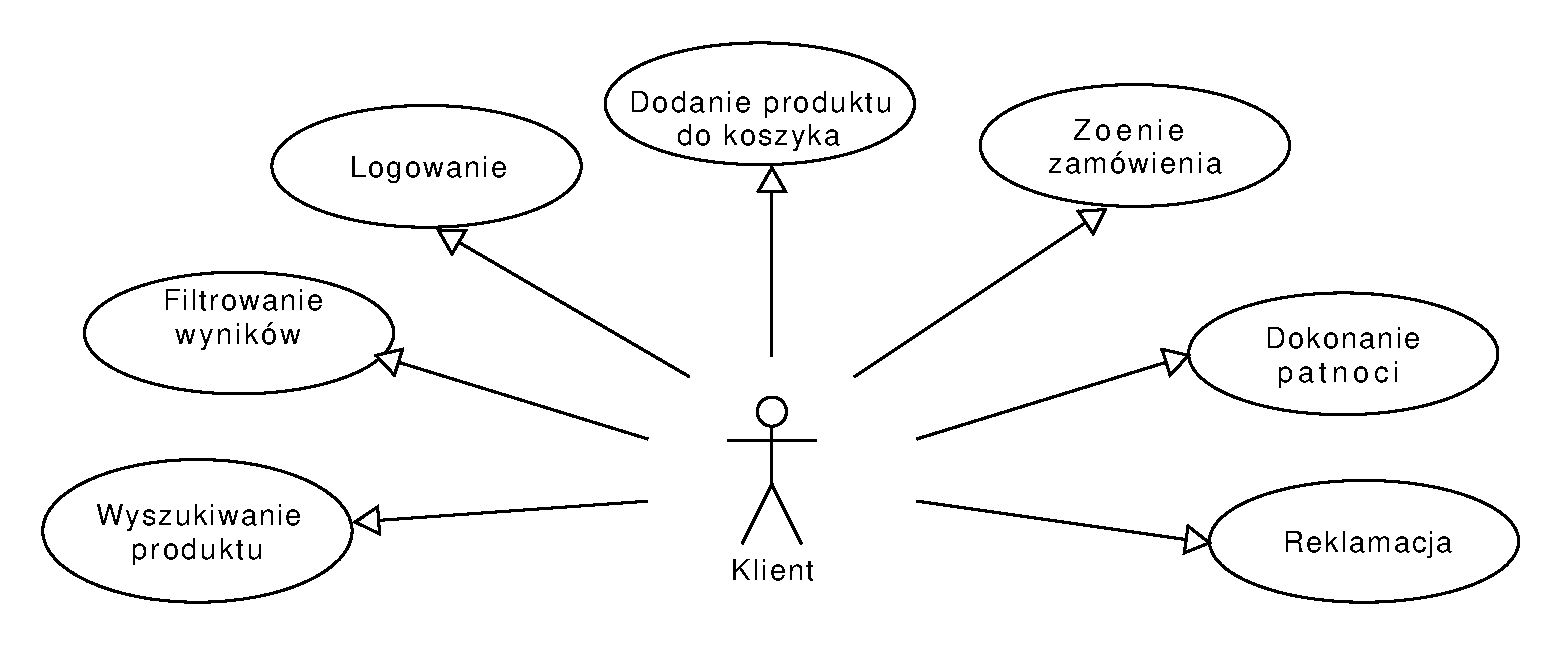
\includegraphics[width=1\textwidth]{uccustomer.pdf}
	\end{center}
	\caption{{\color{black}Diagram przypadków użycia związany z Administratorem ewentualniego systemu.}} \label{useCaseCustomer}
\end{figure}

Diagramy typu \textit{use-case} ściśle wiążą się z wymaganiami funkcjonalnymi systemu. Jest wiadome, że można je również sklasyfikować pod względem aktorów występujących w systemie, dlatego też powiązania przypadków użycia z wymaganiami funkcjonalnymi zostały umieszczone na diagramie z rysunku \ref{wymtoUC}. Na diagram należy patrzeć poziomo, po zapoznaniu się z legendą. Wymagania są w nieprzypadkowej kolejności, są ustawione od lewej do prawej. Im bardziej na prawo, tym wymaganie jest bardziej biznesowe, im bardziej na lewo -- dotyczy rdzeniowych elementów platformy. Warto zauważyć zależność, że im dalej patrzymy na diagram, tym więcej niebieskich i żółtych \textit{use case'ów} -- tych zarezerowowanych dla Administracji i Klientów rozwiązania e-commerce. Natomiast im bardziej na lewo tym więcej czerwonego, czyli przypadków przemyślanych dla Programisty.
\begin{figure}
	\begin{center}
		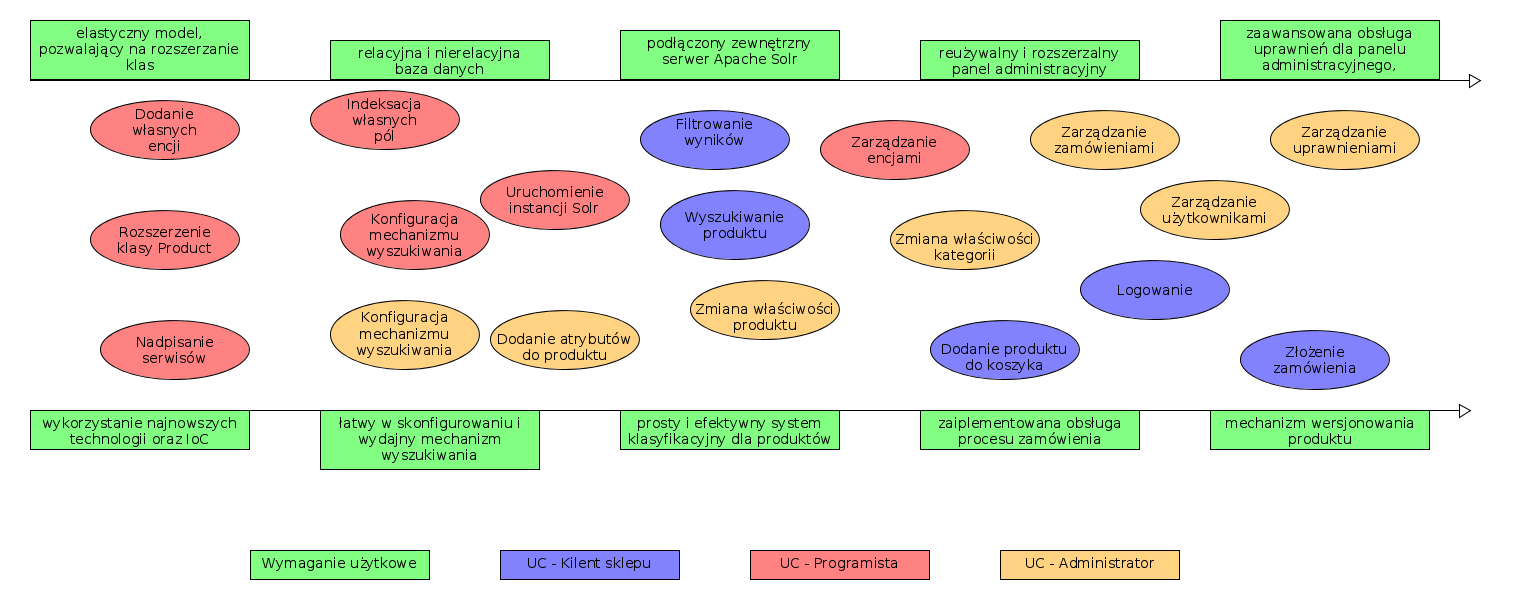
\includegraphics[angle=270,scale=0.4]{wymToUC.png}
	\end{center}
	\caption{{\color{black}Diagram przypadków użycia związany z wymaganiami funkcjonalnymi}} \label{wymtoUC}
\end{figure}

\section{Diagramy aktywności}

W tej sekcji zostały przedstawione diagramy aktywności dla elementów systemu. Aby zachować spójność w rozważaniach podzielono je na trzy grupy: 
\begin{itemize}
	\item diagramy dotyczące budowania rozwiązań e-commerce za pomocą platformy
	\item diagramy dotyczące zarządzania rozwiązaniami e-commerce
	\item diagramy dotyczące przebiegu funkcjinalności biznesowych związanych z kientem końcowym
\end{itemize}  
Jak można zauważyć, te trzy grupy korespondują z aktorami opisywanego rozwiązania, zdefiniowanymi na początku rozdziału. Punkt pierwszy dotyczy Programisty, drugi Administratora, a ostatni Klienta końcowego.

\subsection{Diagramy dotyczące dewelopmentu aplikacji}
Niniejsze diagramy będą opisywały procesy związane z budowaniem rozwiązań opartych na podstawie opisywanego frameworku. 
\begin{figure}[h!]
\begin{center}
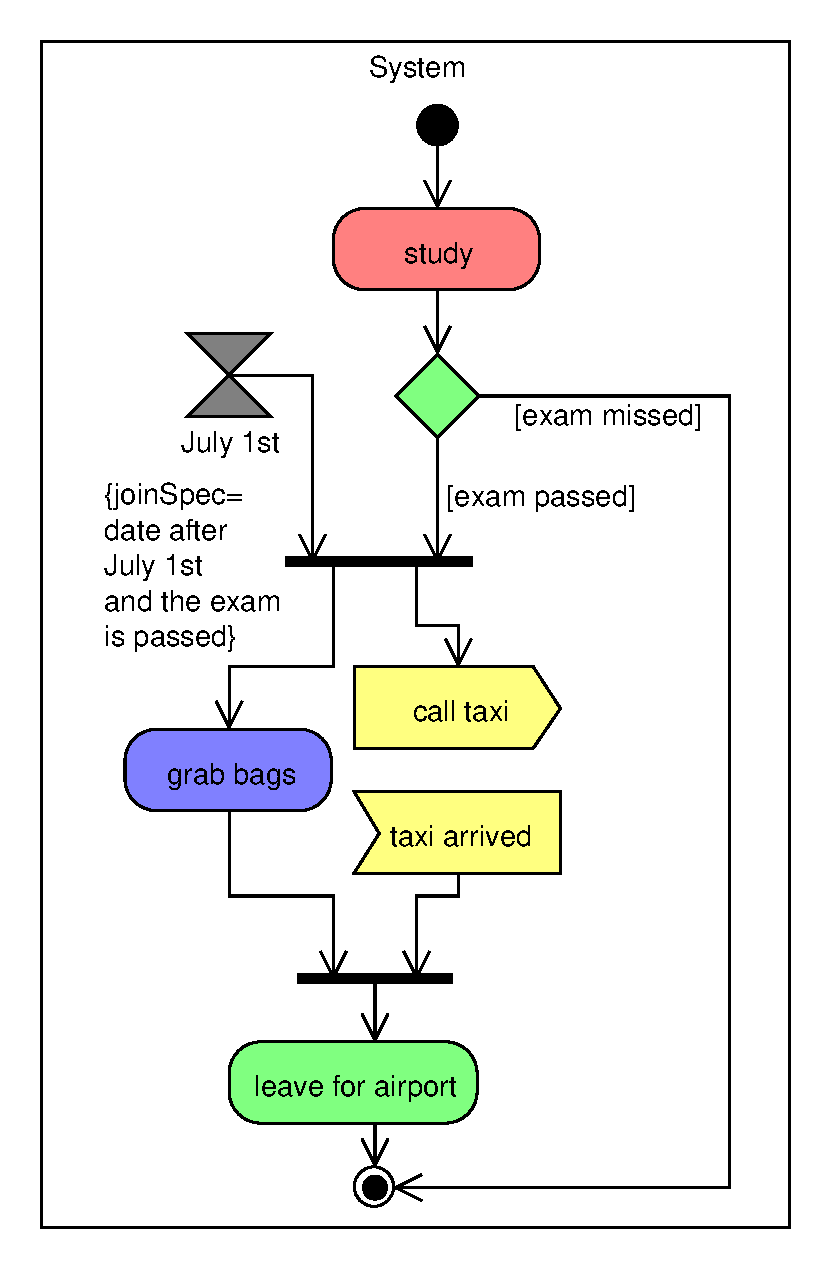
\includegraphics[width=0.5\textwidth]{aktyw.pdf}
\end{center}
\caption{{\color{dgray}Diagram aktywności związany z procesem rejestracji dokumentu.}} \label{czynnosci_GD}
\end{figure}  

\section{Diagramy sekwencji}

W tej sekcji należy przedstawić diagramy sekwencji dla obiektów systemu zidentyfikowanych na podstawie wcześniejszych rozważań. Należy wykorzystać nazewnictwo wprowadzone w poprzednich rozdziałach, w szczególności odpowiadające definicjom wprowadzonych klas.

\section{Diagramy stanów}

W tej sekcji należy przedstawić diagramy stanów w których może znaleźć się system. Diagramy te są szczególnie istotne przy projektowaniu systemów czasu rzeczywistego. 

\section{Diagramy klas}

W tej sekcji należy przedstawić diagramy klas dla odpowiednich elementów systemu zidentyfikowane na podstawie wcześniejszych rozważań

\section{Projekt bazy danych}

W tej sekcji należy przedstawić projekt bazy danych. Należy omówić wycinek rzeczywistości i odpowiadające mu zidentyfikowane elementy systemu, których wartości będą podlegać utrwalaniu. Należy przedyskutować wybór typów danych dla atrybutów poszczególnych obiektów. Należy uzasadnić wybór platformy DBMS. Dla relacyjnych baz danych należy przedyskutować jej normalizację.

\section{Opis protokołów}

W tej sekcji należy omówić protokoły wykorzystywane przez komponenty systemu. Omówić formaty komunikatów i zilustrować je przykładami. 

\section{Opis algorytmów}

W tej sekcji należy wymienić i przedyskutować algorytmy wykorzystywane w systemie. Algorytmy należy przedstawić w pseudokodzie (wykorzystać pakiet \texttt{algorithm2e}). Omówienia poszczególnych kroków algorytmów powinny zawierać odwołania do odpowiednich linii pseudokodu. Dla zaproponowanych autorskich algorytmów należy przeprowadzić analizę ich złożoności czasowej i pamięciowej. 

{\color{dgray}
Algorytm bąblowania jest przedstawiony w Pseudokodzie~\ref{alg:mine}.
}

{\small
\begin{pseudokod}[H]
%\SetAlTitleFnt{small}
\SetArgSty{normalfont}
\SetKwFunction{Process}{Process}
\SetKwFunction{Calculate}{Calculate}
\KwIn{Zbiór bąbli $B$}
\KwOut{Wyporność $W$}
\ForEach{$b \in B$}{
\Process{$b$}\;
\For{$i \leftarrow 1$ \KwTo $|B|$}{
\If{\Calculate{EW($i$,$b$)} $\le$ 0}{
$b \leftarrow 2*b$\;
}
}
}
\While{$B \neq \emptyset$}{
\For{$j \leftarrow 1$ \KwTo $|B|$}{
\If{\Calculate{FT($j$,$\hat{b}$)} $\le 0$}{
$w \leftarrow 2*\hat{b}$\;
$W \leftarrow W \cup \{w\}$\;
$B \leftarrow B \setminus \{b\}$\;
}
}
}
\caption{Wyporność przez bąblowanie}\label{alg:mine}
\end{pseudokod}
}

